%
%
%
%
%
\section{Block-Periodic Residue Sequences}\label{sec:block}
The residue sequences of Section~\ref{sec:residue} carry one exact relation per level: the staggered residue sequence designs one geometric digit at every full level, the residue sequence one skeleton digit at every prefix $P_{sK-1}$. The nets of \cite{Gru26geo} design all $s$ geometric digits of one prefix at once, the whole geometric layer together with its responses at carry depths up to $s-2$%
, and that is how they reach separations $1-O(1/q)$ at the full levels%
. A frame scramble cannot do this at every full level by exact relations: exact relations of bounded depth can design all $s$ geometric digits on at most a fraction $1/s$ of the levels (Section~\ref{sec:count}). It can do it on exactly that fraction. The idea is to spread the $s$ relations over $s$ consecutive digits: every coordinate reads its digits in blocks of $s$, with $s$ different local multipliers, and the residue theorem then installs the complete design of the nets at every $s$-th full level, $m\in s^2\N$. In dimensions two and three this gives $1-2/p$ for every prime $p\ge3$ resp.\ $p\ge5$, with a short proof.

\subsection{The Construction}\label{sec:blockdef}
A \emph{design} in the sense of \cite{Gru26geo} prescribes how the geometric digits depend on the last cell digits: $F_n[i][c]$ is the change of the geometric digit of coordinate $i$ when the cell digit of coordinate $c$ at carry depth $n$ (the finest cell digit is at carry depth $0$) increases by one. We use designs $F=(F_0,\dots,F_{s-2})$ of integer $s\times s$ matrices, read modulo $p$, with partial sums $M^{(j)}=F_0+\dots+F_j$; a carry of length $l$ in coordinate $c$ changes the geometric digits by the column $c$ of $M^{(\min(l,s-1)-1)}$. For places $a_c$ and \emph{row constants} $v\in(\F_p^*)^s$ put $\tau_{ic}=1/(a_i-a_c)$ for $i\ne c$. The design is \emph{reachable} if for every column $c$ and every $n\le s-2$
\[
F_n[i][c]=v_i^{-1}\,\tau_{ic}\,\gamma_{c,n}(\tau_{ic})\qquad(i\ne c)
\]
with a polynomial $\gamma_{c,n}\in\F_p[X]$ of exact degree $n$; the diagonal entries are free. This is the reachability condition of \cite{Gru26geo}%
, with the row constants $v_i^{-1}$ and stated for the individual $F_n$ instead of the partial sums, which is equivalent. Write $u_i=1/(z-a_i)$.

\begin{definition}[Block-periodic residue sequence]\label{def:block}
Let $p\ge s\ge2$ be a prime, $a_0,\dots,a_{s-1}\in\F_p$ distinct places, $\theta\in\F_p^*$, $v\in(\F_p^*)^s$ row constants, $F=(F_0,\dots,F_{s-2})$ a reachable design, and $\ell\ge s$ the \emph{block period}; if $\ell>s$, let also $v'\in(\F_p^*)^s$ be a second check vector. Put $\Omega=w^\ell/\theta$. At each place $a_c$ define $\ell$ \emph{local multipliers} $\varphi_{c,0},\dots,\varphi_{c,\ell-1}$:
\begin{enumerate}
\item[(a)] the \emph{design multipliers} $\varphi_{c,\ell-1-n}$, $0\le n\le s-2$: the rational functions with
\[
u_i=-v_i\sum_{n=0}^{s-2}F_n[i][c]\,\varphi_{c,\ell-1-n}\qquad\text{for every }i\ne c;
\]
\item[(b)] if $\ell>s$, the \emph{skeleton multipliers} $\varphi_{c,j}=w^{\ell-1-j}/v'_c$, $1\le j\le\ell-s$;
\item[(c)] the \emph{own multiplier} $\varphi_{c,0}=v_c^{-1}\,\Omega\,u_c+\Omega\sum_{n=0}^{s-2}F_n[c][c]\,\varphi_{c,\ell-1-n}$.
\end{enumerate}
The \emph{block-periodic residue sequence} is the digital sequence over $\F_p$ with the digits
\[
y_{c,\ell n+j}(V)=\Res_{a_c}\bigl(V\,\varphi_{c,j}\,\Omega^{-(n+1)}dz\bigr),\qquad n\ge0,\ 0\le j<\ell .
\]
\end{definition}

So the digits of each coordinate come in blocks of $\ell$, and multiplying the index by $w^\ell$ shifts every coordinate by one block; for $\ell=1$ this is a self-similar scramble. The generator matrices are again one coefficient per entry, $C_c[\ell n+j][i]=[(z-a_c)^{\ell(n+1)-1}]\,z^i\varphi_{c,j}\,(z-a_c)^{\ell(n+1)}\Omega^{-n-1}$. The system (a) has a unique solution, and the multipliers have the orders of vanishing needed for $t=0$; both are shown in the proof below.

\begin{theorem}[Block-periodic residue sequences]\label{thm:block}
Let $\ell=s$ in Definition~\ref{def:block}.
\begin{enumerate}
\item[(i)] The sequence is a digital $(0,s)$-sequence over $\F_p$.
\item[(ii)] For every $K\ge1$, every coordinate $i$ and every $V$ with $\deg V<s^2K$,
\[
y_{i,sK}(V)=\sum_c\sum_{n=0}^{s-2}F_n[i][c]\,y_{c,sK-1-n}(V):
\]
at every full level $P_{s^2K}$ the geometric digits follow the design exactly.
\item[(iii)] $\sep{P_{s^2K}}\ge\LB(F)$ for every $K\ge1$, where $\LB(F)$ is the one-digit relaxation of Lemma~\ref{lem:cert} ($j=1$) for the carry responses $D(l)=M^{(\min(l,s-1)-1)}$; it is the one-digit relaxation of \cite{Gru26geo}%
\ with a jitter of one unit in every coordinate. The level family is $\Lev=s^2\N$.
\end{enumerate}
In particular, for every $K\ge1$:
\begin{enumerate}
\item[(a)] $s=2$, places $(0,1)$, $v=(1,1)$, $F_0=\bigl(\begin{smallmatrix}-1&1\\-1&-1\end{smallmatrix}\bigr)$: $\sep{P_{4K}}\ge1-2/p$ for every prime $p\ge3$;
\item[(b)] $s=3$, places $(0,2,1)$, $v=(\frac12,\frac12,-1)$, $(F_0,F_1)=(M,J)$ with
\[
M=\begin{pmatrix}-1&-1&1\\1&-1&-1\\-1&1&-1\end{pmatrix},\qquad J=\begin{pmatrix}0&0&-1\\-1&0&0\\0&-1&0\end{pmatrix},
\]
the layer of the three-dimensional nets of \cite{Gru26geo}%
: $\sep{P_{9K}}\ge1-2/p$ for every prime $p\ge5$;
\item[(c)] $s\ge4$, the design $U^*_s$ of \cite{Gru26geo}%
\ moved to the places $0,1,\frac12,\dots,\frac1{s-1}$, with $v=(1,1,2,\dots,s-1)$: $\sep{P_{s^2K}}\ge1-(a^*_s+1)/p$ for every prime $p\ge5a^*_s+4$, where $a^*_s$ is the constant of \cite{Gru26geo}%
\ ($a^*_4=5$, $a^*_5=16$, $a^*_6=43$, $a^*_7=170$). For $s=4$ at every prime $7\le p\le109$ and for $s=5$ at every prime $19\le p\le109$ the value $\LB(F)=1-(a^*_s+1)/p$ holds as well (computer-assisted). Hence $\sep{P_{16K}}\ge1-6/p$ for every prime $p\ge7$ and $\sep{P_{25K}}\ge1-17/p$ for every prime $p\ge19$.
\item[(d)] The diagonal entries of $F$ are free: (i)--(iii) hold for every diagonal. Keep the off-diagonal entries of (c), put $F_0[c][c]=-\delta_c$ and $F_n[c][c]=0$ for $n\ge1$, with $\delta=(3,3,3,3)$, $(7,\dots,7)$, $(3,12,13,14,13,13)$, $(41,44,59,57,56,6,32)$ for $s=4,5,6,7$ (in the order of the places). Then $\sep{P_{s^2K}}$ is at least $1-4/p$, $1-8/p$, $1-15/p$, $1-60/p$ for every prime $p\ge11$, $23$, $37$, $191$, respectively, and $\sep{P_{16K}}\ge\sqrt3/7$ at $p=7$; also $\LB(F)>0$ for $s=5$ at $p=11,13,17,19$, for $s=6$ at every prime $17\le p\le31$, and for $s=7$ at $p=17,19,23$ and every prime $31\le p\le181$ (computer-assisted).
\end{enumerate}
\end{theorem}

\begin{proof}
(i) Fix $c$ and write $\vartheta_n=\varphi_{c,s-1-n}$ for the design multipliers. At $a_c$, $u_i=-\sum_{k\ge0}\tau_{ic}^{k+1}(z-a_c)^k$, so $[(z-a_c)^k]u_i=-\tau_{ic}^{k+1}$. By reachability, (a) reads $u_i=-\sum_n\tau_{ic}\gamma_{c,n}(\tau_{ic})\vartheta_n$, and its matrix $(-\tau_{ic}\gamma_{c,n}(\tau_{ic}))_{i\ne c,\,n\le s-2}$ is invertible: the $\tau_{ic}$ are nonzero and distinct, and the $\gamma_{c,n}$ have exact degrees $0,\dots,s-2$, so the matrix is a diagonal matrix times a triangular change of basis times a Vandermonde matrix. So (a) has a unique solution, a combination of the $u_i$ with constant coefficients. Comparing the coefficients of $(z-a_c)^k$, $k\le s-2$, gives $\tau^k=\sum_n\gamma_{c,n}(\tau)\,[(z-a_c)^k]\vartheta_n$ at the $s-1$ distinct nodes $\tau=\tau_{ic}$, hence as an identity of polynomials of degree at most $s-2$. Expanding $\tau^k$ in the triangular basis $(\gamma_{c,n})$ shows $[(z-a_c)^k]\vartheta_n=0$ for $k<n$ and $[(z-a_c)^n]\vartheta_n\ne0$: $\vartheta_n$ vanishes to order exactly $n$ at $a_c$, i.e.\ $\varphi_{c,j}$ to order exactly $s-1-j$. The own multiplier vanishes to order exactly $s-1$: $v_c^{-1}\Omega u_c=v_c^{-1}w_cw^{s-1}/\theta$ does, and the other terms vanish to order at least $s$. As $\Omega$ vanishes to order exactly $s$ at $a_c$, the differential $\varphi_{c,j}\Omega^{-n-1}dz$ has a pole of order exactly $s(n+1)-(s-1-j)=sn+j+1$ there. So digit $sn+j$ is the residue of $V$ against a polar differential of exact order $sn+j+1$, and Lemma~\ref{lem:resform}(a) and Lemma~\ref{lem:t0} give $t=0$.

(ii) By (c) with $\ell=s$, $y_{i,sK}(V)=v_i^{-1}\Res_{a_i}(Vu_i\Omega^{-K}dz)+\sum_nF_n[i][i]\,y_{i,s(K-1)+s-1-n}(V)$. The rational function $Vu_i\Omega^{-K}$ has its finite poles at the places, and degree at most $(s^2K-1)-1-s^2K=-2$; by Lemma~\ref{lem:resform}(c) its residues add up to $0$. At $a_c$, $c\ne i$, (a) replaces $u_i$ by $-v_i\sum_nF_n[i][c]\varphi_{c,s-1-n}$, so $\Res_{a_c}(Vu_i\Omega^{-K}dz)=-v_i\sum_nF_n[i][c]\,y_{c,s(K-1)+s-1-n}(V)$. Hence $v_i^{-1}\Res_{a_i}(Vu_i\Omega^{-K}dz)=\sum_{c\ne i}\sum_nF_n[i][c]\,y_{c,sK-1-n}(V)$, which together with the own terms is the claim.

(iii) At the full level $P_{s^2K}$ each coordinate has $sK$ cell digits, and its geometric digit is $y_{\cdot,sK}$. By (ii) it depends only on the cell digits at carry depths $0,\dots,s-2$, through $F$; adding $1$ to the $l$ finest cell digits of coordinate $c$ changes it by column $c$ of $M^{(\min(l,s-1)-1)}$, at every level and for every carry length, the wrap included. These responses do not depend on $K$, so Lemma~\ref{lem:cert} with $j=1$ gives $\sep{P_{s^2K}}\ge\LB(F)$ for every $K$ (as $p^{sK}\ge4$). In $\LB(F)$ a moving coordinate whose change $\sigma_i$ is backward, $e_i\sigma_i\le0$ with $|\sigma_i|<p$, contributes $f_1(e_i,\sigma_i)=c_{|\sigma_i|+1}$, $c_j:=1-j/p$ (Remark~\ref{rem:onedigit}); every other coordinate contributes at least $0$.

(a) $F_1$ is absent, so the carry length does not matter, and $\sigma=e_0F_0[\cdot][0]+e_1F_0[\cdot][1]$. The axis steps give $\sigma=\mp(1,1)$ and $\sigma=\pm(1,-1)$: the moving coordinate is backward with $|\sigma|=1$, a term $c_2=1-2/p$. The diagonal steps give $\sigma=\pm(0,-2)$ and $\pm(-2,0)$, the terms $(c_1^2+c_3^2)^{1/2}\ge c_2$. So $\LB(F)=1-2/p$ for every prime $p\ge3$. Reachability needs only nonzero crosses for $s=2$.

(b) Reachability, by hand over $\mathbb{Q}$: in column $c=0,1,2$ the values $v_iM[i][c]/\tau_{ic}$ ($i\ne c$) are $1,1$; $1,1$; $-\frac12,-\frac12$, so $\gamma_{c,0}$ is constant; the values $v_iJ[i][c]/\tau_{ic}$ are $(-1,0)$, $(0,-1)$, $(\frac12,0)$ at two distinct nodes, so $\gamma_{c,1}$ has degree exactly $1$. All numbers are $0,\pm1,\pm2,\pm\frac12$, so this holds over $\F_p$ for every prime $p\ge3$. With $\omega_d=1$ if the carry length in coordinate $d$ is at least $2$ and $\omega_d=0$ otherwise, the changes are $\sigma_i=-e_i-e_{i+1}+(1-\omega_{i+2})e_{i+2}$ (indices modulo $3$), exactly as for the nets of \cite{Gru26geo}%
. The sign analysis there%
, which uses only this formula, $|\sigma_i|\le3<p$ and at least two cell digits per coordinate, shows: an axis step has $\sigma_i=-e_i$; a step with two moving axes has two backward coordinates with $|\sigma|\le1$ and $|\sigma|\le2$; a step with three moving axes has either a backward coordinate with $|\sigma|=3$ and another with $|\sigma|\le1$, or a forward coordinate and two backward ones with $|\sigma|\le1$ and $|\sigma|\le2$, or three backward coordinates with $|\sigma|\le2$. With the jitter of one unit also on the axis steps this gives
\[
\LB(F)=\min\bigl(c_2,\ (c_2^2+c_3^2)^{1/2},\ (c_2^2+c_4^2)^{1/2},\ \sqrt3\,c_3\bigr)=\min(c_2,\sqrt3\,c_3)=c_2=1-\tfrac2p\quad(p\ge5),
\]
since $\sqrt3(1-3/p)\ge1-2/p$ exactly when $p\ge(3\sqrt3-2)/(\sqrt3-1)\approx4.37$.

(c) \emph{Reachability.} By \cite{Gru26geo}%
, $U^*_s$ is reachable at the places $\hat a_c\in\{\infty,0,1,\dots,s-2\}$ with constant row scalars: $M^{(j)}[c][d]=\tilde w_{cd}\,\tilde g_{d,j}(\tilde y_{cd})$ ($c\ne d$, $j\le s-2$), where $\tilde g_{d,j}$ has degree $j$, coefficients in $\Z[1/(s-2)!]$ and a leading coefficient whose prime factors are at most $s-2$, and $\tilde w_{cd}=\tilde y_{cd}=1/(\hat a_c-\hat a_d)$ for finite $\hat a_c,\hat a_d$, $\tilde w_{\infty d}=1$, $\tilde y_{\infty d}=0$, $\tilde w_{c\infty}=1$, $\tilde y_{c\infty}=\hat a_c$. Move the places by $x\mapsto1/(x+1)$, so $a_c=1/(\hat a_c+1)$ ($a_c=0$ for $\hat a_c=\infty$), and let $\tau_{cd}=1/(a_c-a_d)$. For finite $\hat a_c,\hat a_d$, $\tau_{cd}=-(\hat a_c+1)(\hat a_d+1)\tilde y_{cd}$, and $(\hat a_c+1)\tilde y_{cd}=1+(\hat a_d+1)\tilde y_{cd}$; hence
\[
\tilde y_{cd}=A_d(\tau_{cd}):=-\frac{\tau_{cd}}{(\hat a_d+1)^2}-\frac1{\hat a_d+1},\qquad \tilde w_{cd}=\varrho_c\,\tau_{cd}\,\varsigma_d,\quad \varrho_c=-\frac1{\hat a_c+1},\ \varsigma_d=\frac1{\hat a_d+1},
\]
an affine function of $\tau_{cd}$ whose coefficients depend on the column only. For $\hat a_c=\infty$: $\tau_{\infty d}=-(\hat a_d+1)$, $A_d(\tau_{\infty d})=0=\tilde y_{\infty d}$ and $\tilde w_{\infty d}=1=\varrho_\infty\tau_{\infty d}\varsigma_d$ with $\varrho_\infty=-1$. For $\hat a_d=\infty$: $\tau_{c\infty}=\hat a_c+1$, so $\tilde y_{c\infty}=A_\infty(\tau_{c\infty})$ with $A_\infty(X)=X-1$, and $\tilde w_{c\infty}=\varrho_c\tau_{c\infty}\varsigma_\infty$ with $\varsigma_\infty=-1$. Therefore $M^{(j)}[c][d]=\varrho_c\,\tau_{cd}\,\varsigma_d\tilde g_{d,j}(A_d(\tau_{cd}))$, a polynomial in $\tau_{cd}$ of exact degree $j$ times $\tau_{cd}$, for every prime $p\ge s$ (then $\hat a_d+1\in\{1,\dots,s-1\}$ and the leading coefficients are units, and the places are distinct). Differences of consecutive partial sums give the individual $F_n$, so the design is reachable with $v_c^{-1}=-\varrho_c$ after a change of sign of all $\gamma$, i.e.\ $v=(1,1,2,\dots,s-1)$ in the order $\hat a=(\infty,0,\dots,s-2)$.

\emph{The bound.} $U^*_s$ has the diagonal $F_0[c][c]=-\alpha_c$ and zero diagonal at the carry depths $n\ge1$, and it is diagonally dominant: $\alpha_c\ge\sum_{d\ne c}\max_j|M^{(j)}[c][d]|$, with $a^*_s=\max_c\alpha_c$ \cite{Gru26geo}%
. An axis step along $c$ has $\sigma_c=-e_c\alpha_c$, a term $1-(\alpha_c+1)/p\ge1-(a^*_s+1)/p$. On a step with at least two moving axes every moving coordinate is backward with $|\sigma_i|\le2a^*_s<p$, so the step has at least two terms $c_{2a^*_s+1}$, and $\sqrt2(p-2a^*_s-1)\ge p-a^*_s-1$ for $p\ge(3+\sqrt2)a^*_s+1$, in particular for $p\ge5a^*_s+4$. This is the diagonal dominance argument of \cite{Gru26geo}%
\ with a jitter of one unit on the axis steps. So $\LB(F)\ge1-(a^*_s+1)/p$ for $p\ge(3+\sqrt2)a^*_s+1$ (for $s=6$, $7$ from $p=191$, $757$ on), with equality when a row with $\alpha_c=a^*_s$ has the other entries of its column of $F_0$ in $\{-1,0,1\}$, since its axis step then attains the bound. The coordinate of the place $0$ (the place $\infty$ of \cite{Gru26geo}) has such a column for every $s$: at carry depth $0$ its column is a multiple of $(\tilde w_{c\infty})_c=(1,\dots,1)$, and $U^*_s$ takes $(1,\dots,1)$%
; for $s\le10$ it has $\alpha_c=a^*_s$ (exact computation). As the entries of $F_0$ off the diagonal are nonzero integers, $\alpha_c\ge s-1$, so $p\ge5a^*_s+4$ implies $p\ge s$.

\emph{Small primes.} $\LB(F)$ is a minimum over finitely many configurations (steps, and carry lengths capped at $s-1$), and the reachability above holds for every prime $p\ge s$. Its exact value at every prime $7\le p\le109$ ($s=4$) and $19\le p\le109$ ($s=5$) is $1-(a^*_s+1)/p$; with $5a^*_4+4=29$ and $5a^*_5+4=84$ this covers every prime $p\ge7$ resp.\ $p\ge19$ (only the lower bound needs the computation). Part (d) is proved after Lemma~\ref{lem:signclass}.
\end{proof}

\emph{The free diagonal.} The diagonal of $U^*_s$ is chosen for diagonal dominance, which the nets need: on every step every moving coordinate is backward. The sequence never uses the diagonal: reachability and the system (a) involve only the entries $F_n[i][c]$, $i\ne c$, and in the own multiplier (c) the diagonal terms carry the factor $\Omega$. But $\LB(F)$ is set by the worst step, and the axis step along $c$ pays $\alpha_c+1$. A smaller diagonal softens this step, as long as every other step keeps one short backward coordinate or two backward ones. Figure~\ref{fig:freediag} shows the gain. Here changes are computed in the integers, $\sigma=\sum_ce_cM^{(\min(l_c,s-1)-1)}[\cdot][c]$, and a moving coordinate $i$ is backward if $e_i\sigma_i\le0$.

\begin{figure}[t]
\centering
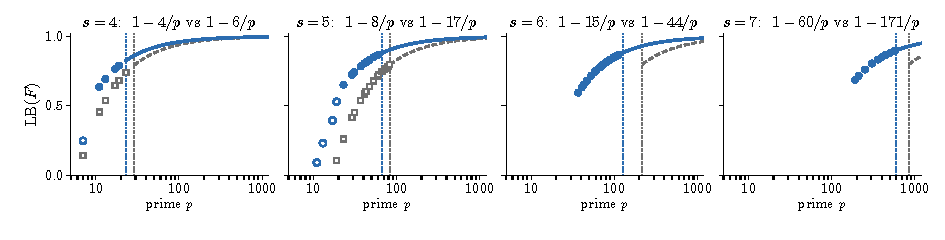
\includegraphics[width=\linewidth]{fig_freediag.pdf}
\caption{$\LB(F)$ of Theorem~\ref{thm:block} against $p$. Grey: $U^*_s$ (dashed: $1-(a^*_s+1)/p$, written proof for $p\ge5a^*_s+4$; squares: exact values, c.a.). Blue, all c.a.: the free diagonal of (d) (solid: $1-(A+1)/p$ past the threshold of Lemma~\ref{lem:signclass}; dots: exact values below it; circles: the quoted values at $p=7$, $11\le p\le19$). Dotted: the thresholds. In Lean for $s=4,5,6$ (from $p=11$, $23$, $125$), not for $s=7$.}
\label{fig:freediag}
\end{figure}

\begin{lemma}[Backward coordinates]\label{lem:signclass}
Let $F$ be a design with partial sums $M^{(j)}$, let $A\ge0$ be an integer, and let $S=\max_i\sum_c\max_j|M^{(j)}[i][c]|$. Suppose that every step $e$, with every choice of carry lengths, has a backward moving coordinate with $|\sigma_i|\le A$ or two backward moving coordinates. Then $\LB(F)\ge1-(A+1)/p$ for every prime $p>S$ with $(p-A-1)^2\le2(p-S-1)^2$.
\end{lemma}

\begin{proof}
For $p>S$ every change has $|\sigma_i|\le S<p$, so a backward coordinate contributes $c_{|\sigma_i|+1}$ (proof of Theorem~\ref{thm:block}(iii)). The term of the step is at least $c_{A+1}$ in the first case and at least $\sqrt2\,c_{S+1}\ge c_{A+1}$ in the second.
\end{proof}

The hypothesis does not depend on $p$ and is a finite check. Diagonal dominance is the case in which every moving coordinate is backward; for $U^*_s$ ($A=a^*_s$, $S\le2a^*_s$) the lemma gives the range $p\ge(3+\sqrt2)a^*_s+1$ above.

\begin{proof}[Proof of Theorem~\ref{thm:block}(d)]
Reachability is that of (c). The hypothesis of Lemma~\ref{lem:signclass} holds with $A=3$, $7$, $14$, $59$ and $S=8$, $23$, $46$, $211$ (exhaustive check, computer-assisted), which gives $\LB(F)\ge1-(A+1)/p$ for every prime $p\ge23$, $67$, $127$, $587$. Below these primes $\LB(F)$ was evaluated exactly at every prime of the stated ranges (computer-assisted; for $s=5$ it is $1/11$, $3/13$, $3\sqrt5/17$, $\sqrt{101}/19$ at $p=11,\dots,19$), and Theorem~\ref{thm:block}(iii) applies. For $s=4,5$ the bound is attained by the axis step at the place $0$ (its column of $F_0$ is $(1,\dots,1)$ off the diagonal, and $\delta_0=A$), for $s=6$ by the axis step at the place $\frac13$ with carry length $4$.
\end{proof}

How far can the diagonal go? With the off-diagonal entries of $U^*_s$ fixed, the least $A$ in Lemma~\ref{lem:signclass} gives $\lim_{p\to\infty}p(1-\LB(F))=A+1$ (a step whose only backward coordinate has $|\sigma_i|=A$ has the term $1-(A+1)/p+O(p^{-2})$). An axis step forces $0\le\delta_c\le A$, and an exhaustive search over $\delta\in[0,A]^s$ finds no diagonal with $A\le2$, $6$, $13$ for $s=4,5,6$ (computer-assisted): in this sense $4$, $8$, $15$ are optimal. For $s=7$, $60$ is the best found, against $a^*_7+1=171$.

For $s=4$ the design of Theorem~\ref{thm:block}(c) is, in the order of the places $0,1,\frac12,\frac13$ and with $v=(1,1,2,3)$,
\[
F_0=\begin{pmatrix}-5&2&1&2\\1&-3&-1&-1\\1&2&-5&-2\\1&1&1&-3\end{pmatrix},\quad
F_1=\begin{pmatrix}0&-3&-1&-1\\-2&0&2&1\\-1&-1&0&3\\0&-1&0&0\end{pmatrix},\quad
F_2=\begin{pmatrix}0&2&0&-1\\2&0&-2&0\\0&-1&0&-2\\-1&0&-1&0\end{pmatrix};
\]
the largest diagonal entry is $a^*_4=5$, and the design of (d) replaces the diagonal of $F_0$ by $-3$. Table~\ref{tab:block} collects the data. Figure~\ref{fig:block} shows the case $s=2$, $p=7$ inside and outside the family.

\begin{table}[t]
\centering
\footnotesize
\caption{The block-periodic residue sequences of Theorem~\ref{thm:block} ($\Lev=s^2\N$). Places and row constants: $(0,1)$, $(1,1)$ for $s=2$; $(0,2,1)$, $(\frac12,\frac12,-1)$ for $s=3$; $(0,1,\frac12,\dots,\frac1{s-1})$, $(1,1,2,\dots,s-1)$ for $s\ge4$. ``$U^*_s$, $\delta$'': $U^*_s$ off the diagonal, $F_0[c][c]=-\delta_c$. ``proof'': written proof; ``c.a.'': computer-assisted (exact $\LB(F)$, and for (d) Lemma~\ref{lem:signclass}); each for every prime in the range; in parentheses, further primes with $\LB(F)>0$.}
\label{tab:block}
\setlength{\tabcolsep}{4pt}
\begin{tabular}{@{}c l l l l@{}}
\toprule
$s$ & design & $\LB(F)$ & proof & c.a.\\
\midrule
2 & $F_0=\bigl(\begin{smallmatrix}-1&1\\-1&-1\end{smallmatrix}\bigr)$ & $1-2/p$ & $p\ge3$ & --\\
3 & $(M,J)$, Thm.~\ref{thm:block}(b) & $1-2/p$ & $p\ge5$ & --\\
4 & $U^*_4$ (above) & $1-6/p$ & $p\ge29$ & $7\le p\le109$\\
5 & $U^*_5$ & $1-17/p$ & $p\ge84$ & $19\le p\le109$\\
$\ge4$ & $U^*_s$ & $1-(a^*_s+1)/p$ & $p\ge5a^*_s+4$ & --\\
4 & $U^*_4$, $\delta=(3,3,3,3)$ & $1-4/p$ & -- & $p\ge11$ ($7$)\\
5 & $U^*_5$, $\delta=(7,7,7,7,7)$ & $1-8/p$ & -- & $p\ge23$ ($11$--$19$)\\
6 & $U^*_6$, $\delta=(3,12,13,14,13,13)$ & $1-15/p$ & -- & $p\ge37$ ($17$--$31$)\\
7 & $U^*_7$, $\delta=(41,44,59,57,56,6,32)$ & $1-60/p$ & -- & $p\ge191$ ($17$--$23$, $31$--$181$)\\
\bottomrule
\end{tabular}
\end{table}

\begin{figure}[t]
\centering
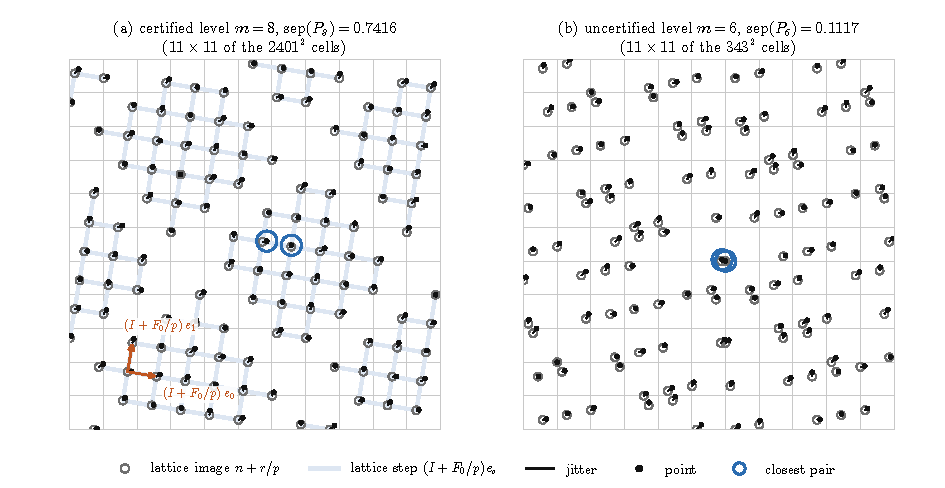
\includegraphics[width=0.9\linewidth]{fig_block.pdf}
\caption{The block-periodic residue sequence of Theorem~\ref{thm:block}(a), $s=2$, $p=7$, places $(0,1)$, $\theta=1$ (exact points). (a)~The full level $m=8$ ($2401\times2401$ cells), $11\times11$ cells around the closest pair: each point (dot) lies within one unit of the last digit of its lattice image $n+r/p$ (open circle); where no geometric digit wraps, neighbouring lattice images differ by a column of $I+F_0/p$ (light segments): patches of $\Z^2$ rotated by $\arctan(1/6)$, scaled by $\sqrt{37}/7\approx0.87$, separated by slip planes. Exact $\sep{P_8}=0.7416$ ($0.7613$ at $m=4$), certified bound $1-2/7=0.7143$. (b)~The full level $m=6$, which is not in the family $4\N$: its geometric digits are not designed, and the closest pair is only $0.1117$ cell units apart (exact).}
\label{fig:block}
\end{figure}

\begin{remark}[Exact separations and the levels in between]\label{rem:blockexact}
Exact values (illustration only) are close to the certified ones: for $s=2$, $\sep{P_4}=0.5730$, $\sep{P_8}=\sep{P_{12}}=0.3862$ and $\sep{P_{16}}=0.3610$ at $p=3$ (bound $1/3$); $0.6237$ at $m=4,8$ for $p=5$ (bound $0.6$); $0.8383$, $0.8604$, $0.8909$, $0.9016$, $0.9177$ at $m=4$ for $p=11$, $13$, $17$, $19$, $23$; for $s=3$, $\sep{P_9}=0.6211$ at $p=5$ ($\theta=1$; bound $0.6$) and $0.7378$ at $p=7$ (bound $0.7143$); at $p=3$, where the bound of (b) is $0$, $\sep{P_9}=0.4381$. Outside the family the separation is not controlled: for $s=2$, $p=5$ the levels $m=2,3,5,6,7,9,10$ have $0.368$, $0.366$, $0.276$, $0.159$, $0.354$, $0.092$, $0.159$ (evidence, not a claim).
\end{remark}

\emph{All $N$.} The family $s^2\N$ has largest gap $s^2$, so Lemma~\ref{lem:prefix} gives $\delta(P_{[N]})N^{1/s}\ge\LB(F)\,p^{-s}$ for every $N\ge2$ and the mesh ratio $h/\delta\le\sqrt s\,p^{s+1}/\LB(F)$: these sequences are quasi-uniform, the strongest of our constructions \emph{at} their certified sizes, but for all $N$ weaker than the residue sequences of Section~\ref{sec:residue}, whose bound $\LB/p$ is larger whenever $p>2^s$ (for $s=2$, $p=5$: $0.024$ against $0.089$).

\emph{The lost $1/p$.} The nets of \cite{Gru26geo} with the layer $(M,J)$ reach $1-1/q$ at every full level for $q\ge8$%
. The difference is the axis step: in the nets the deeper digits of a coordinate do not depend on its own cell%
, so an axis step has no jitter in the moving coordinate; here it has, and $1-1/p$ becomes $1-2/p$. Whether free data in the scramble can restore $1-1/p$ is open.

\subsection{Two Level Families from One Scramble}\label{sec:blocktwo}
With a block period $\ell>s$ the scramble has $\ell-s$ local multipliers left over. Giving them to a second check vector adds skeleton relations of the residue sequence at most levels in between.

\begin{theorem}[Two level families from one scramble]\label{thm:blocktwo}
Let $\ell>s$ in Definition~\ref{def:block}, with the second check vector $v'$. Then:
\begin{enumerate}
\item[(i)] the sequence is a digital $(0,s)$-sequence over $\F_p$;
\item[(ii)] for every $K\ge1$ and $\deg V<s\ell K$, $y_{i,\ell K}(V)=\sum_c\sum_{n=0}^{s-2}F_n[i][c]\,y_{c,\ell K-1-n}(V)$, and $\sep{P_{s\ell K}}\ge\LB(F)$;
\item[(iii)] for every $T\equiv1,\dots,\ell-s\pmod\ell$ and $\deg V\le s(T+1)-2$, $\sum_cv'_c\,y_{c,T}(V)=0$, and $\sep{P_{s(T+1)-1}}\ge p^{-1/s}\ljit(\Lambda_{v'})$.
\end{enumerate}
So one scramble is certified on the design levels $m\in s\ell\N$, with the constants of Theorem~\ref{thm:block}, and on the skeleton levels $m=s(T+1)-1$, $T\equiv1,\dots,\ell-s\pmod\ell$, with those of Theorem~\ref{thm:residue}: a fraction $1/\ell$ of the full levels and a fraction $(\ell-s)/\ell$ of the levels $m\equiv-1\pmod s$. For instance $s=2$, $\ell=4$: design levels $8\N$, skeleton levels $3,5,11,13,19,21,\dots$; $s=2$, $\ell=3$: $6\N$ and $3,9,15,\dots$; $s=3$, $\ell=4$: $12\N$ and $5,17,29,\dots$.
\end{theorem}

\begin{proof}
(i) As in Theorem~\ref{thm:block}(i), with $\Omega$ of order $\ell$: the design multipliers vanish to the orders $0,\dots,s-2$, the skeleton multipliers $w^{\ell-1-j}/v'_c$ to the orders $\ell-1-j\in\{s-1,\dots,\ell-2\}$, and the own multiplier to the order $\ell-1$. So $\varphi_{c,j}$ vanishes to order exactly $\ell-1-j$ for every $j$, digit $\ell n+j$ is the residue against a polar differential of exact order $\ell n+j+1$, and Lemma~\ref{lem:t0} applies.
(ii) The proof of Theorem~\ref{thm:block}(ii),(iii) is unchanged: it uses only (a), (c) and $\deg(Vu_i\Omega^{-K})\le-2$, which holds for $\deg V<s\ell K$; at $P_{s\ell K}$ the geometric digit is digit $\ell K$.
(iii) Write $T=\ell n+j$ with $1\le j\le\ell-s$. Then $v'_cy_{c,T}(V)=\Res_{a_c}(Vw^{\ell-1-j}\Omega^{-n-1}dz)=\theta^{n+1}\Res_{a_c}(Vw^{-T-1}dz)$, and by Lemma~\ref{lem:resform}(c) these add up to $0$ when $\deg V\le s(T+1)-2$. This is the skeleton relation of Lemma~\ref{lem:residue-rel} at level $T+1$ with the check vector $v'$. The proof of Theorem~\ref{thm:residue} uses only $t=0$ and this relation, so it gives the bound.
\end{proof}

The trade-off is set by $\ell$: $\ell=s$ is Theorem~\ref{thm:block}; as $\ell$ grows, almost all levels $m\equiv-1$ are certified with the constants of the residue sequence, and the full design appears on a sparser family. Exact computations agree with both bounds, e.g.\ for $s=2$, $\ell=4$, $p=5$, $v'=(2,4)$: $\sep{P_m}=0.5999$, $0.6264$, $0.4995$ at the skeleton levels $m=3,5,11$ (bound $0.4472$) and $0.6787$ at the design level $m=8$ (bound $0.6$). For all $N$ the largest gap between certified levels is still of order $s^2$ (exactly $s^2-s+1$, for every $\ell>s$), so Lemma~\ref{lem:prefix} gives no improvement over the residue sequence.

\subsection{A Skeleton Relation Implied by the Design}\label{sec:implied}
Even with $\ell=s$ the design can carry a skeleton relation at the level just after the design level, provided its diagonal is chosen for it.

\begin{proposition}[A skeleton relation implied by the design]\label{prop:implied}
In Definition~\ref{def:block} (any $\ell\ge s$), let $\bar v\in(\F_p^*)^s$ satisfy
\[
\bar v_i=\xi\,v_i/w'(a_i)\quad\text{for one }\xi\in\F_p^*,\qquad\text{and}\qquad \bar v^{\mathsf T}F_n\equiv0\pmod p\quad\text{for every }n\le s-2 .
\]
Then $\sum_i\bar v_i\,y_{i,\ell K}(V)=0$ for every $K\ge0$ and every $V$ with $\deg V\le s(\ell K+1)-2$: the skeleton relation with check vector $\bar v$ holds at the level $m=s(\ell K+1)-1$, in addition to the design at $m=s\ell K$. Consequently $\sep{P_{s(\ell K+1)-1}}\ge p^{-1/s}\ljit(\Lambda_{\bar v})$ for every $K\ge0$.
\end{proposition}

\begin{proof}
Keep the coefficient at infinity in the proof of Theorem~\ref{thm:block}(ii): by Lemma~\ref{lem:resform}(c), for every $V$,
\[
y_{i,\ell K}(V)=\sum_c\sum_{n=0}^{s-2}F_n[i][c]\,y_{c,\ell K-1-n}(V)+v_i^{-1}\,[z^{-1}]\bigl(Vu_i\Omega^{-K}\bigr)
\]
(for $K=0$ the sum is empty). Multiply by $\bar v_i$ and sum over $i$. The double sum vanishes because $\bar v^{\mathsf T}F_n\equiv0$. By partial fractions $\sum_iu_i/w'(a_i)=1/w$, so the rest is $\xi[z^{-1}](V\Omega^{-K}/w)=\xi\theta^K[z^{-1}](V/w^{\ell K+1})$, which is $0$ for $\deg V\le s(\ell K+1)-2$. The bound follows as in Theorem~\ref{thm:residue}.
\end{proof}

The condition $\bar v^{\mathsf T}F_n\equiv0$ can always be met by the free diagonal, choosing $F_n[c][c]$ with $\bar v_cF_n[c][c]=-\sum_{i\ne c}\bar v_iF_n[i][c]$. But it has a price. It says that every column of every $F_n$, read as an integer vector of centred residues, lies in $\Lambda_{\bar v}$. Hence
\[
\ljit(\Lambda_{\bar v})\ \le\ \min\bigl\{\|(|F_n[\cdot][c]|-\mathbf 1)_+\|_2:\ n\le s-2,\ F_n[\cdot][c]\ne0\bigr\},
\]
so a good implied skeleton relation (with $\ljit(\Lambda_{\bar v})$ of order $p^{1/s}$) forces an entry of order $p^{1/s}$ in every nonzero column of the design, far from the entries $\pm1$ of the nets. (For example a column $(-2,-1)$ forces $\ljit\le1$.) In dimension two the price can be paid exactly at the primes one more than a square.

\begin{corollary}[Primes of the form $u^2+1$]\label{cor:gauss}
Let $p=u^2+1$ be a prime ($u$ even: $p=5,17,37,101,197,257,401,\dots$), $s=\ell=2$, places $(0,1)$, $v=(-u,-1)$ and $F_0=\bigl(\begin{smallmatrix}-1&u\\-u&-1\end{smallmatrix}\bigr)$. Then for every $K\ge1$
\[
\begin{aligned}
\sep{P_{4K}}&\ \ge\ \frac{\sqrt{(u-2)^2+(u^2-u-1)^2}}p\ \ge\ 1-\frac{\sqrt{p-1}+2}p,\\
\sep{P_{4K+1}}&\ \ge\ \frac{u-1}{\sqrt p}=\frac{\sqrt{p-1}-1}{\sqrt p}.
\end{aligned}
\]
The fine cells occupied by $P_{4K+1}$ form the square lattice $\Z(1,u)+\Z(u,-1)$.
\end{corollary}

\begin{proof}
For $s=2$ reachability only asks for nonzero crosses. With $w=z^2-z$, $w'(0)=-1$, $w'(1)=1$, the vector $\bar v=(u,-1)$ satisfies $\bar v_i=v_i/w'(a_i)$, and $\bar v^{\mathsf T}F_0=(-u+u,\,u^2+1)\equiv0$. \emph{Design levels.} The carry length does not matter, and the four steps give $\sigma=(-1,-u)$, $(u,-1)$, $(u-1,-u-1)$ and $(-u-1,1-u)$. The axis steps have the terms $\bigl((p-2)^2+(u-1)^2\bigr)^{1/2}/p\ge(p-2)/p$. On the diagonal steps the two coordinates contribute $(u-2)/p$ and $(p-u-2)/p=(u^2-u-1)/p$, and $(p-2)^2-(p-u-2)^2-(u-2)^2=2pu-2u^2-4>0$, so the diagonal term is the minimum; it is at least $(p-u-2)/p$. \emph{Skeleton levels.} By Proposition~\ref{prop:implied} the skeleton relation with $\bar v$ holds at $m=4K+1$. The lattice $\Lambda_{\bar v}=\{b:ub_0\equiv b_1\}$ contains $(1,u)$ and $(u,-1)$, whose determinant is $-p$, so they span it, and $|m(1,u)+n(u,-1)|^2=(m^2+n^2)p$. The four vectors $\pm(1,u)$, $\pm(u,-1)$ have $\|(|b|-\mathbf 1)_+\|_2=u-1$, and every other nonzero vector has length at least $\sqrt{2p}$, hence $\|(|b|-\mathbf 1)_+\|_2\ge\sqrt{2p}-\sqrt2\ge u-1$. So $\ljit(\Lambda_{\bar v})=u-1$, and Theorem~\ref{thm:residue} applies.
\end{proof}

At the skeleton levels $\bar v=(u,-1)$ is the Korobov vector of Corollary~\ref{cor:korobov} ($\rho=u$), so the bound is the Korobov bound $(\rho-1)p^{-1/2}$ of the residue sequence; it is about $1-p^{-1/2}$, against the general lower form $1-2p^{-1/2}$, because the fine-cell lattice is an exact square. It is the best over all check vectors at $p=5$, $17$, $37$, $197$, not at $p=101$, $257$, $401$, where other check vectors have a larger $\ljit^2$ ($85$, $241$, $369$ against $81$, $225$, $361$; exact computation). At the design levels the constant is $1-O(p^{-1/2})$, below the $1-2/p$ of Theorem~\ref{thm:block}(a): the price of the implied relation. Exact computations agree: $\LB(F)=0.6576$, $0.7912$, $0.8847$ at $p=17$, $37$, $101$, against $\sep{P_4}=0.6597$, $0.8072$, $0.8885$; at the skeleton level $m=5$, $\sep{P_5}=0.6406$, $0.7988$, $0.9094$ at $p=5$, $17$, $37$, against $0.4472$, $0.7276$, $0.8220$.

\begin{remark}[Meeting the density bound]\label{rem:gaussfrontier}
For $s=2$ and $\ell\ge3$, adding the skeleton multipliers of Theorem~\ref{thm:blocktwo} to the design of Corollary~\ref{cor:gauss} certifies the design at $m\in2\ell\N$ and the skeleton relation at the levels $m=2N+1$ with $N\not\equiv-1\pmod\ell$, i.e.\ at a fraction $(\ell-1)/\ell$ of the levels $m\equiv1\pmod2$ (Theorem~\ref{thm:blocktwo}(iii) and Proposition~\ref{prop:implied}). The two densities add up to $1$, the largest value that exact relations of bounded depth allow (Corollary~\ref{cor:density}). The bound for all $N$ does not improve on that of the residue sequence: the largest gap between certified levels is $3$, against $2$ for the residue sequence.
\end{remark}
